\graphicspath{{img/intro/out}}


\chapter{Introduction}
\label{ch:intro}

\section{Artificial Intelligence}
\label{sec:artificial-intelligence}
Artificial Intelligence (AI) is a broad subject of study that can be defined in different ways~\cite[chapter 1]{russell_artificial_2021}.
John McCarthy, often called the “father of AI”\cite{wiki_ai_2023, woo_fatherofai_2014, andresen_fatherofai_2002}, defines it as “the science and engineering of making intelligent machines”~\cite{stanford-whatisai}, where intelligence means “the computational part of the ability to achieve goals in the world”~\cite{stanford-whatisai}.
AI is sometimes mistakenly used interchangeably with Machine Learning.
Machine learning is a subset of AI concerned with enabling AI systems to learn from experience~\cite[chapter 1]{russell_artificial_2021}.
Machine learning enables the development of large-scale AI systems as they are used today.
\\
The study of artificial intelligence was first proposed by McCarthy et al. in late 1955 \cite{mccarthy_proposal_1955}.
It went through two major hype cycles in the sixties and the eighties~\cite{googlengram_ai, wiki_ai_2023, sitnflash_history_2017} followed by phases of “AI winter”.
The current (as of early 2024) AI boom, sometimes also called “AI spring”~\cite{aispring} was started by groundbreaking advances in speech recognition~\cite{hinton_deep_2012} and image classification~\cite{krizhevsky_imagenet_2012} in 2012~\cite{google_decade_2021, house_2012_2019} and reached the general public at the latest in late 2022, following the release of ChatGPT~\cite{openai_chatgpt_intro}, a multipurpose AI-chatbot, open to everyone~\cite{openai_chatgpt}.
\\
These breakthroughs are made possible mainly by advancements in the field of machine learning, enabling AI systems to learn from huge amounts of data.
In addition, the exponential increase in computation and storage capabilities as predicted by Moore’s Law~\cite{mooreslaw}, algorithms like backpropagation~\cite{rumelhart_learning_1986} allowed incorporating large amounts of data into machine learning models in realistic amounts of time.
\\
Today, AI systems are indispensable in many areas such as web search engines~\cite{google_howweuseai}, recommendation systems~\cite{burke_recommender_2011}, human speech recognition and generation~\cite{elevenlabs, hinton_deep_2012}, image recognition and generation~\cite{midjourney, krizhevsky_imagenet_2012} and personal assistants~\cite{openai_chatgpt_intro} and surpasses humans in high level strategy games like go and chess~\cite{silver_mastering_2016, silver_mastering_2017} as well as other videogames~\cite{piper_ai_2019}.

\section{Neural Networks}
\label{sec:neural-networks}
\subsection{Overview}
\label{subsec:overview}
At the heart of almost all the technologies mentioned in the last paragraph are deep artificial neural networks.
The next section will outline the mathematical details of how these systems work and learn.
Although the comparison of artificial neural networks, from now on just called “neural networks”, to their biological counterpart can be criticized as oversimplifying the inner workings of biological brains~\cite[chapter 1.1]{aggarwal_neural_2018}, the architecture of neural networks is heavily inspired by how decision-making and learning work in the human brain~\cite[chapter 1.1]{aggarwal_neural_2018, mit_nnexplained}.
I will illustrate the basic principles of neural networks at the example of a network that detects the gender of a person by looking at pictures.
\\
\\
A neural network consists of a number of layers of artificial neurons, called \textit{nodes}.
In a \textit{fully connected} network, each node is connected to every node in the next layer.
The connection strengths are called \textit{weights}.
An image of a person can be fed into the network by setting the \textit{activation} values of the first layer of the network, the \textit{input layer}, to the individual pixel values of the image.
This information is then fed forward through the layers of the network until the \textit{output layer} is reached.
If a network has at least one layer in between the input and output layer, it is called a \textit{deep neural network}.
These intermediate layers are called \textit{hidden layers}.
If the outputs of each layer are only connected to the inputs of the next layer, the network is called a \textit{feedforward neural network}.
If \textit{feedback} connections are allowed, the network is called a \textit{recurrent neural network}.
\\
In our example, the output layer should consist of only two nodes.
If the activation of the first node is larger than the activation of the second node, the network thinks that the person in the picture is a male.
If on the other hand the second node has a larger activation, the network classifies this person as female~\cite[chapter 1.2]{aggarwal_neural_2018}.
\\
\\
In order to make accurate predictions, a reasonable set of network parameters (i.e.the weights) has to be found.
This is done by training the network with pre-classified images.
After an image has been processed by the network, the output is compared to the correct classification and the network parameters are updated in a way that would improve the networks output if the same image was to be processed again~\cite[chapter 1.2]{aggarwal_neural_2018,ibm_nn}.
\\
This is similar to how humans learn from experience.
If we were to misclassify a persons gender, the unpleasant social experience that may come with that mistake would cause us to update our internal model of what different genders look like so as to not make the same mistake again.
\\
\\
One of the main strengths of neural networks is their ability to \textit{generalize}~\cite{gonfalonieri_understand_2020}.
When a network was trained on a large enough set of examples, it gains the ability to generalize this knowledge to examples that were previously unseen.
The gender classification network from our example doesn't just memorize the genders of the people it has seen, but instead learns about the features that help to identify the gender of a random person.
\\
\\
The problem of image classification is a rather complex one.
One wouldn't typically think of it as finding a function that maps the values of each input pixel to the classification output.
But even very complex problems can be modeled by equally complex functions.
The universal approximation theorem states, that a feedforward neural network with at least one hidden layer with appropriate activation functions (see~\ref{subsubsec:activation-functions} for details) can approximate any continuous function if given enough nodes~\cite[chapter 6.4.1]{goodfellow_deep_2016}.
That's why training a neural network can be thought of as fitting the network to the training data.
\\
\subsection{Mathematical Details}
\label{sec:nn-mathematical-details}
The following section will outline the mathematical details of how neural networks work.
The definitions and derivations are based on~\cite[chapter 1.2-1.3]{aggarwal_neural_2018},~\cite[chapter 5-6]{goodfellow_deep_2016},~\cite{ibm_nn} as well as~\cite[chapter 4.4]{haykin_neural_1998}.
\\
\\
The most complete treatment of the mathematical details of neural networks is arguably given by the framework of computational graphs~\cite{bettilyon_computationalgraphs_2020}.
In this framework, a neural network is treated as single that maps a set of input values to a set of output values.
This funcion is composed of individual mathematical operations and can be represented as a directed graph \cite[section 1.4]{haykin_neural_1998}.
I will not rigorously define the framework of computational graphs here, as this is beyond the scope of this thesis.
Instead, I will explain the priciples of neural networks starting from a single neuron and then build up to a fully connected neural network. 
\subsubsection{Notation}
\label{subsubsec:nn-notation}
The following notation will be used throughout this section:
\begin{equation*}
    \begin{array}{ll}
    \bm{x} & : \text { input vector of the neural network} \\
    \bm{a} & : \text { activation vector of a layer} \\
    \bm{z} & : \text { pre-activation vector of a layer} \\
    \bm{y} & : \text { output vector of the neural network} \\
    \bm{b} & : \text { bias vector of a layer} \\
    x_i, a_i, z_i, y_i, b_i & : \text { individual elements of the respective vectors, for individual nodes } \\
    \bm{w_i} & : \text { weight vector of all weights connected to neuron i} \\
    w_{ij} & : \text { weight of the connection from neuron i of a layer to neuron j of the previous layer } \\
    W & : \text { weight matrix of a layer. Contains rows $\bm{w_i}$} \\
    ^{[J]} & : \text { superscript denoting the layer of a variable} \\
    \end{array}
\end{equation*}
\subsubsection{Single Node}
\label{subsubsec:single-neuron}
\begin{figure}
    \centering
    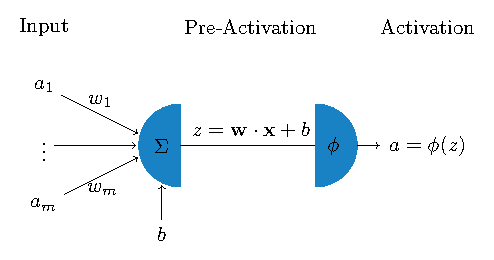
\includegraphics[width=0.5\textwidth]{single_neuron}
    \caption{A single node of a neural network. To get the activation $a$ of the node, the pre-activation $z$ is calculated from the inputs $a_i$ and the bias $b$ and is passed through an activation function $\phi$.}
    \label{fig:single-neuron}
\end{figure}
Before we can build a neural network out of nodes, we have to define how a single node works.
Each node receives the activations $a_i$ from the nodes of the previous layer as inputs. 
Each connection is assigned a weight $w_i$, stored in the node's weight vector $\bm{w}$.
\\
Additionally, each node has a so-called \textit{bias} $b$. 
The bias shifts the net input of the node by a constant value.
It is needed to model certain problems where part of the prediction is independent of the input \cite[6]{aggarwal_neural_2018}.
Examples include all problems where the output should not be zero even if all inputs are zero. 
\\
\\
The net input, called \textit{pre-activation value} $z$ of a node is the weighted sum of all inputs plus the bias:
\begin{equation}
    z = \sum_{i=1}^{m} w_i a_i + b = \bm{w} \cdot \bm{a} + b \text{.}
    \label{eq:pre-activation}
\end{equation}
The pre-activation value is then passed through an \textit{activation function} $\phi$ to get the activation $a$ of the node, which is then passed on to the next layer, where the process is repeated:
\begin{equation}
    a = \phi(z) \text{.}
    \label{eq:activation}
\end{equation}
The whole process is illustrated in figure \ref{fig:single-neuron}.

\subsubsection{Activation Functions}
\label{subsubsec:activation-functions}
The activation function $\phi$ is used to introduce non-linearity into the network and thus increasing its modeling power \cite[section 1.2.1.3]{aggarwal_neural_2018}. 
Some activation functions are also referred to as \textit{squashing function}~\cite[10]{haykin_neural_1998}, as they map the unbounded pre-activation value $z$ to a bounded activation value $a$.
The choice of activation function has a large impact on the performance of the network in terms of both accuracy and speed \cite{dubey_activation_2022}.
The type of function heavily influences the way that information is processed by the network and the complexity of the function naturally has a large impact on the computational cost of the network.
The best choice therefore depends on the problem that is being solved and the architecture of the network.
Typically, the same activation function is used for all nodes in a layer and is applied to the pre-activation value of each node individually, but different layers can use different activation functions depending on their purpose \cite[174]{goodfellow_deep_2016}.
For a long time, the most popular activation functions were (\cite[chapter 6.3]{goodfellow_deep_2016}, \cite[section 1.2.1.3]{aggarwal_neural_2018}) the sigmoid function:
\begin{equation}
    \phi(z) = \sigma(z) = \frac{1}{1+e^{-z}}
    \label{eq:sigmoid}
\end{equation}
and the hyperbolic tangent function:
\begin{equation}
    \phi(z) = \tanh(z) = \frac{e^z - e^{-z}}{e^z + e^{-z}} = 2\sigma(2z) - 1
    \label{eq:tanh}
\end{equation}
as well as the sign function:
\begin{equation}
    \phi(z) = \text{sign}(z) = \begin{cases}
        1 & \text{if } z > 0 \\
        0 & \text{if } z = 0 \\
        -1 & \text{if } z < 0 \text{.}
    \end{cases}
    \label{eq:sign}
\end{equation}
The sign function can map neural network output to a binary classification, but it is not suitable for backpropagation (see section \ref{subsec:backprop}) due to its derivative being zero almost everywhere.
The sigmoid function and the hyperbolic tangent function are both differentiable and limit the output to the range $(-1, 1)$ and $(0, 1)$ respectively.
They are however more computationally expensive than other activation functions and suffer from the \textit{vanishing gradient problem}.
The vanishing gradient problem is caused by the fact that the derivative of the sigmoid function approaches zero for large absolute values of $z$.
This leads to the weights of the nodes in the first layers of the network being updated very slowly, as the gradient of the loss function with respect to the weights of these nodes is very small (see section \ref{subsec:backprop})\cite[section 1.4.2]{aggarwal_neural_2018}\cite{dubey_activation_2022}.
The sigmoid function and the hyperbolic tangent function can be seen in figure \ref{fig:sigmoid} and \ref{fig:tanh}.
\begin{figure}
    \centering
    \begin{subfigure}[b]{0.45\textwidth}
        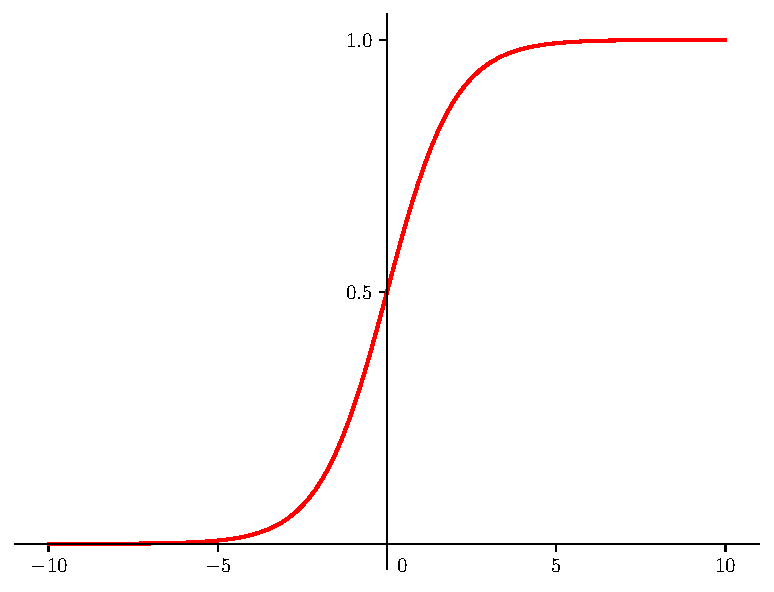
\includegraphics[width=\textwidth]{sigmoid}
        \caption{The sigmoid activation function.}
        \label{fig:sigmoid}
    \end{subfigure}
    \hfill
    \begin{subfigure}[b]{0.45\textwidth}
        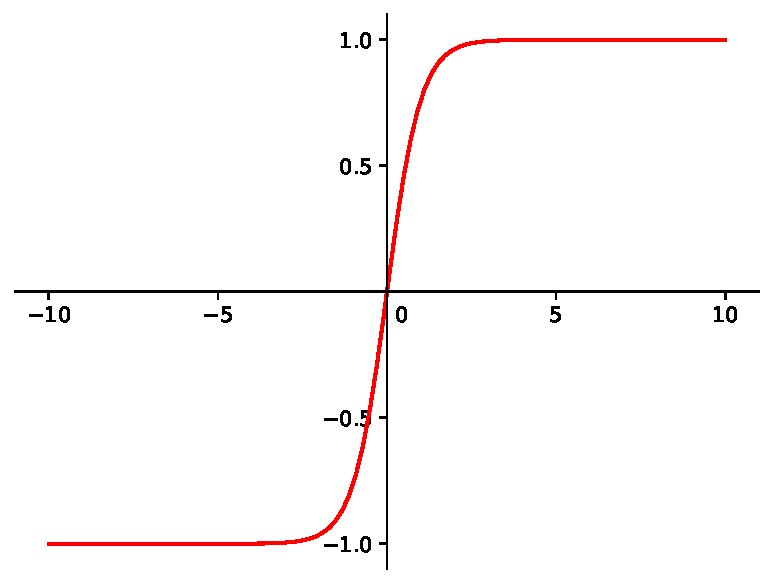
\includegraphics[width=\textwidth]{tanh}
        \caption{The hyperbolic tangent activation function.}
        \label{fig:tanh}
    \end{subfigure}
    \caption{The most popular activation functions before the rise of ReLU.}
    \label{fig:tanhsigmoid}
\end{figure}
\\
\\
In recent years, the \textit{rectified linear unit} (ReLU) and similar stepwise linear functions have become the go-to activation functions for deep neural networks~\cite[chapter 6.3.2]{goodfellow_deep_2016}\cite{dubey_activation_2022}.
ReLU is defined as:
\begin{equation}
    \phi(z) = \max(0, z) = \begin{cases}
        0 & \text{if } z \leq 0 \\
        z & \text{if } z > 0 \text{.}
    \end{cases}
    \label{eq:relu}
\end{equation}
Its main advantage is its very low computational cost, as it consists of only a single comparison. 
Although it is not as prone to the vanishing gradient problem as the sigmoid and the hyperbolic tangent, the problem still exists for negative values of $z$. 
This has been addressed by variations like \textit{Leaky ReLU}, introducing a small but non-zero slope for negative values~\cite{dubey_activation_2022}:
\begin{equation}
    \phi(z) = \max(0.01 z, z) = \begin{cases}
        0.01 z & \text{if } z \leq 0 \\
        z & \text{if } z > 0 \text{.}
    \end{cases}
    \label{eq:leaky-relu}
\end{equation}
The ReLU function and its leaky version can be seen in figures \ref{fig:relu} and \ref{fig:leaky-relu}.
\begin{figure}
    \centering
    \begin{subfigure}[b]{0.45\textwidth}
        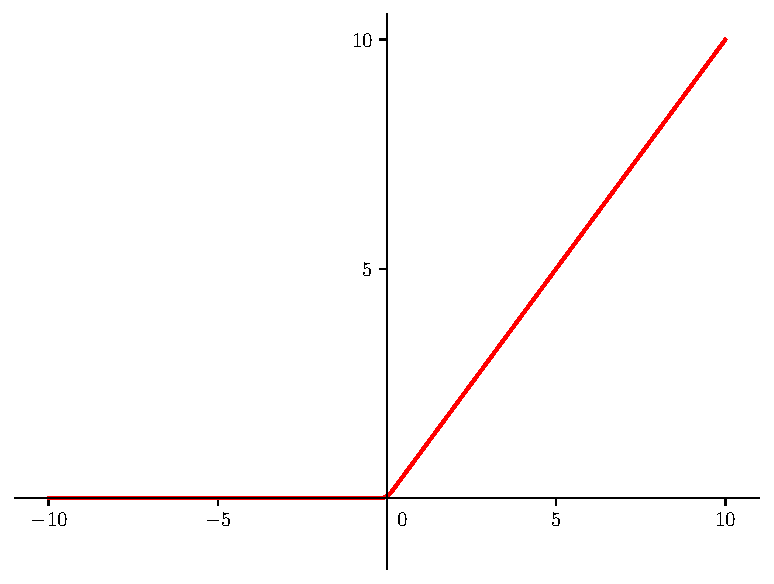
\includegraphics[width=\textwidth]{relu}
        \caption{The rectified linear unit (ReLU) activation function.}
        \label{fig:relu}
    \end{subfigure}
    \hfill
    \begin{subfigure}[b]{0.45\textwidth}
        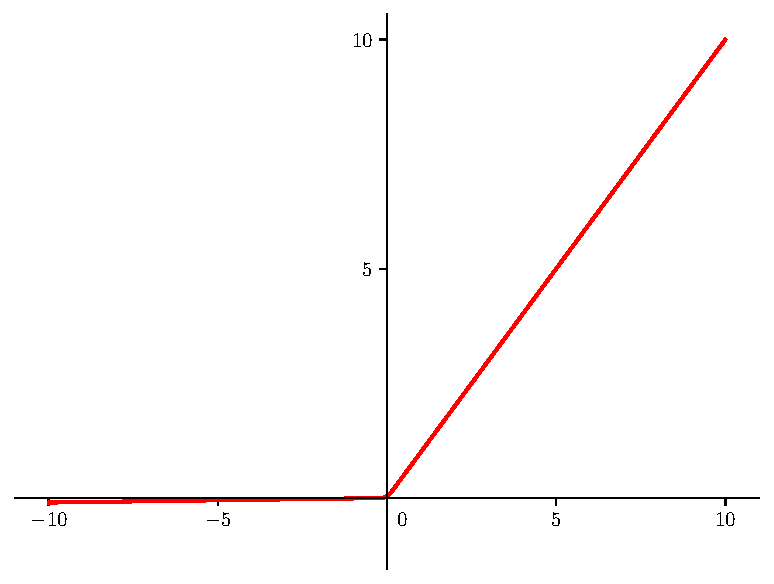
\includegraphics[width=\textwidth]{leaky_relu.pdf}
        \caption{The leaky rectified linear unit (Leaky ReLU) activation function.}
        \label{fig:leaky-relu}
    \end{subfigure}
    
    \caption{Modern, stepwise linear activation functions.}
    \label{fig:subfigures}
\end{figure}


\subsubsection{Forward-Propagation in Feedforward Neural Networks}
\label{subsubsec:forward-propagation}
\begin{figure}
    \centering
    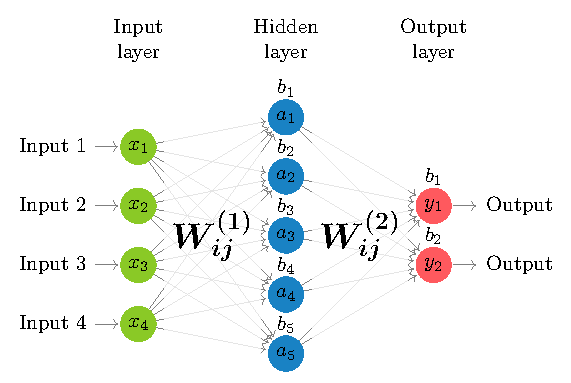
\includegraphics[width=0.9\textwidth]{nn}
    \caption{A feedforward neural network with one hidden layer.}
    \label{fig:nn}
\end{figure}
Now that the workings of the nodes are defined, we can build a fully connected neural network out of these building blocks. 
I will illustrate the process at the example of a feedforward neural network as defined in section \ref{subsec:overview}.
An example of such a network can be seen in figure \ref{fig:nn}. 
\\
\\
The process of feeding an input vector $\bm{x}$ through the network to get the output vector $\bm{y}$ is called \textit{forward-propagation}, as the information propagates through the network layer by layer. The activation of any layer $\bm{a}^{[J]}$ can be calculated from the activation of the previous layer $\bm{a}^{[J-1]}$ by generalizing equation \ref{eq:pre-activation} and \ref{eq:activation} to the vector case:
\begin{equation}
    z_k^{[J]} = \sum_{i=1}^{m} w_{ki}^{[J]} a_i^{[J-1]} + b_k^{[J]} \implies \bm{z}^{[J]} = W^{[J]} \bm{a}^{[J-1]} + \bm{b}^{[J]} \text{,}
    \label{eq:pre-activation-vector}
\end{equation}
\begin{equation}
    a_k^{[J]} = \phi(z_k^{[J]}) \implies \bm{a}^{[J]} = \phi(\bm{z}^{[J]}) \text{,}
    \label{eq:activation-vector}
\end{equation}
where the activation function $\phi: \mathbb{R}^m \rightarrow \mathbb{R}^m$ is applied element-wise.
The activation of the input layer $\bm{a}^{[0]}$ is simply the input vector $\bm{x}$ and the activation of the output layer $\bm{a}^{[L]}$ is the output vector $\bm{y}$.
\\
\\
Equations \ref{eq:pre-activation-vector} and \ref{eq:activation-vector} can be applied recursively to calculate the activation of each layer from the input layer to the output layer:
\begin{align}
    \bm{y} = \bm{a}^{[L]} &= \phi(W^{[L]} \bm{a}^{[L-1]} + \bm{b}^{[L]}) \\
    &= \phi(W^{[L]} \phi(W^{[L-1]} \bm{a}^{[L-2]} + \bm{b}^{[L-1]}) + \bm{b}^{[L]}) \\
    &= \phi(W^{[L]} \phi(W^{[L-1]} \phi(\dots \phi(W^{[1]} \bm{x} + \bm{b}^{[1]}) \dots) + \bm{b}^{[L-1]}) + \bm{b}^{[L]}) \text{.}
    \label{eq:forward-propagation}
\end{align}
This equation also shows the significance of the activation function. 
Without it, the whole network would be equivalent to a single layer and could be replaced by a single matrix multiplication.
It would therefore only be able to model linear functions. 
To show this, let's set $\phi(z)$ to the identity in equation \ref{eq:forward-propagation}. This yields:
\begin{align}
    \bm{y} &= W^{[L]} W^{[L-1]} \dots W^{[1]} \bm{x} + \bm{b}^{[L]} + W^{[L]} \bm{b}^{[L-1]} + \dots + W^{[L]} W^{[L-1]} \dots W^{[2]} \bm{b}^{[1]} \\
    &= \widetilde{W} \bm{x} + \tilde{\bm{b}} \text{.}
    \label{eq:linear-network}
\end{align}

\subsubsection{Loss Functions and Gradient Descent}
\label{subsubsec:loss-functions}
In order to produce meaningful output, the network's weights and biases have to be adjusted to minimize the error of the network's output.
This process is called \textit{training} the network.
The error of the network is measured by a \textit{loss function} $\lambda(\bm{y}, \bm{\hat{y}})$, where $\bm{\hat{y}}$ is some target output vector.
The loss function is a measure of how far the network's output $\bm{y}$ is from the target output $\bm{\hat{y}}$.
As we want to minimize the networks error, the training process is esentially an optimization problem \cite[chapter 4.3]{goodfellow_deep_2016}.
Let's step back from neural networks for a moment and look at a method to minimize a function $f(\bm{x})$ with respect to it's parameters $\bm{x}$.
The most common method to do this in machine learning is \textit{gradient descent} \cite[chapter 4.3]{goodfellow_deep_2016}.
\\
\\
\begin{figure}
    \centering
    \begin{subfigure}[b]{0.45\textwidth}
        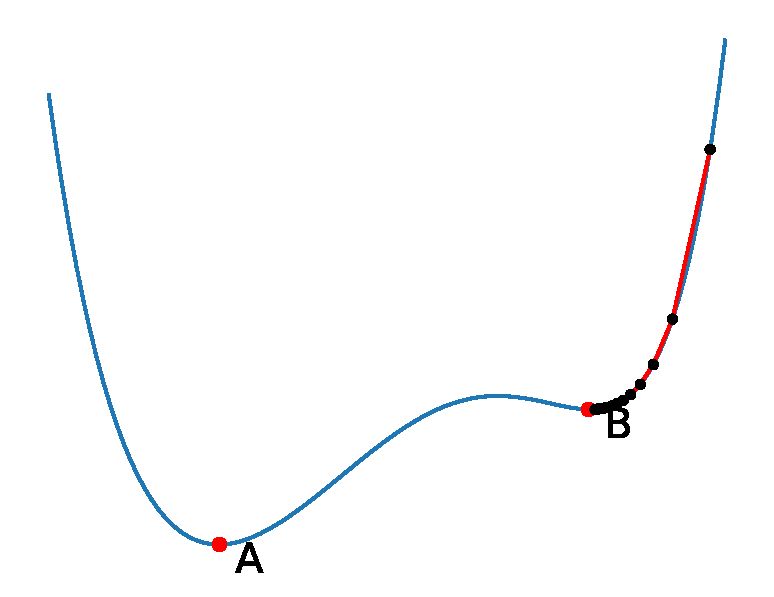
\includegraphics[width=\textwidth]{gradient_descent_small_lr}
        \caption{Gradient descent with a small learning rate.}
        \label{fig:gradient-descent-small}
    \end{subfigure}
    \hfill
    \begin{subfigure}[b]{0.45\textwidth}
        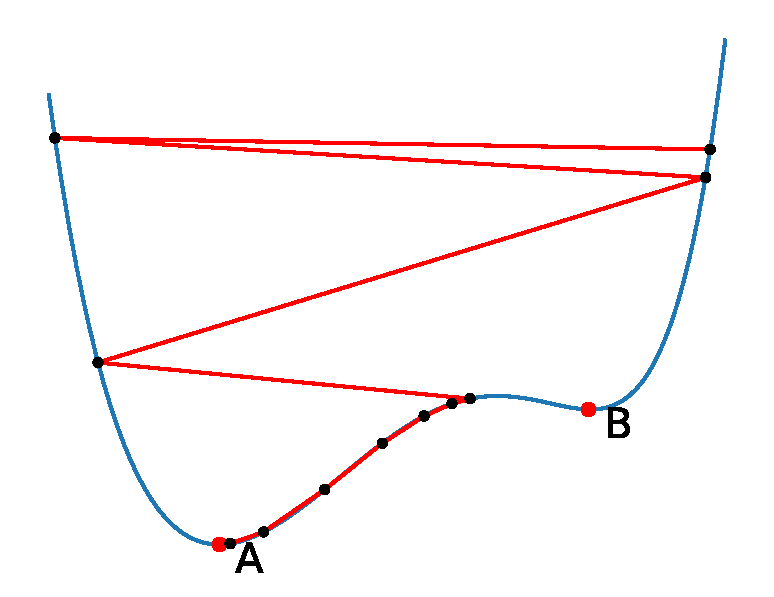
\includegraphics[width=\textwidth]{gradient_descent_large_lr}
        \caption{Gradient descent with a large learning rate.}
        \label{fig:gradient-descent-large}
    \end{subfigure}
    \caption{Gradient descent with different learning rates. Choosing the learning rate too small can lead to slow convergence and to being stuck in local minima. Choosing the learning rate too large can lead to \textit{overshooting} and to the algorithm diverging. Here, the algorithm still converges, but the large oscillations slow down the convergence.}
    \label{fig:gradient-descent}
\end{figure}
If we imagine the function $f(\bm{x})$ as a landscape, the goal of gradient descent is to find the lowest point of the landscape.
To do this, the algorithm starts at some point $\bm{x}_0$ and in each iteration, it takes a step in the direction of steepest descent. 
The size of the step is determined by the \textit{learning rate} $\eta$.
Choosing an appropriate learning rate is crucial for the algorithm to converge.
Figure \ref{fig:gradient-descent} shows gradient descent with different learning rates and the resulting paths through the landscape.
\\
\\
As is known from multivariable calculus, the direction of steepest descent of a function $f(\bm{x})$ is given by the negative gradient $\nabla f(\bm{x})$.
We can therefore update the parameters $\bm{x}$ in each iteration by:
\begin{equation}
    \bm{x}_{n+1} = \bm{x}_n - \eta \nabla f(\bm{x}_n) \text{.}
    \label{eq:gradient-descent}
\end{equation}
After a sufficient number of iterations, the algorithm will converge to a local minimum of the function. 
In the region around the minimum, the gradient is close to zero and the algorithm will not change the parameters significantly anymore.
We therefore define a threshold $\epsilon$ and stop the algorithm if the norm of the gradient falls below this threshold. 
The gradient descent algorithm is summarized in algorithm \ref{alg:gradient-descent}.
\begin{algorithm}
    \caption{Gradient Descent}
    \label{alg:gradient-descent}
    \begin{algorithmic}[1]
        \renewcommand{\algorithmicensure}{\textbf{Output:}}
        \Require
            \Statex $f(\bm{x})$: Function to minimize
            \Statex $\eta$: Learning rate
            \Statex $\epsilon$: Threshold
            \Statex $\bm{x}_0$: Initial parameters
        \Ensure $\bm{x^*}=\arg\min f(\bm{x})$: Parameters that minimize $f(\bm{x})$
        \output{$\bm{x\star}=\arg\min f(\bm{x})$: Parameters that minimize $f(\bm{x})$}
        \Statex
        \State $\bm{x} \gets \bm{x}_0$ \Comment{Initialize parameters}
        \While{$\norm{\nabla f(\bm{x}_n)} > \epsilon$} \Comment{Until convergence}
            \State $\bm{x} \gets \bm{x} - \eta \nabla f(\bm{x})$ \Comment{Update parameters}
        \EndWhile
        \State \Return $\bm{x}$ \Comment{Return parameters}
    \end{algorithmic}
\end{algorithm}

Going back to neural networks, the function that we want to minimize is the loss function $\lambda(\bm{y}, \bm{\hat{y}})$. 
As the loss function depends on the network's output $\bm{y}$, which in turn depends on the network's parameters $\bm{w}$ and $\bm{b}$, the loss function is a function of the network's parameters $\lambda(\bm{w}, \bm{b})$. 
\\
\\
For single layer networks, the calculation of the gradients is straightforward. 
For multi-layer networks however, the loss function depends on the parameters of ealier layers in a non-trivial way. 
The next section will outline an algorithm, that allows the efficient calculation of the gradients of multi-layer networks.

\subsubsection{The Backpropagation Algorithm}
\label{subsec:backprop}
% Goodfellow Ch. 6.5
% Aggarwal Ch. 1.3
% Jonas BA
The calculation of the gradients is the most computationally expensive part of training a neural network. The invention of the \textit{backpropagation} algorithm by Rumelhart et al. in 1986~\cite{rumelhart_learning_1986} was a major breakthrough in the field of neural networks, as it allowed very efficient gradient calculation and thus enabled the training of large neural networks. 
\\
The idea behind backpropagation is to propagate the error back through the network after each forward-propagation step using \textit{local gradients} $\delta$.
During the forward-propagation step, the activations of each layer are stored in memory and used to calculate the derivatives need for the backpropagation step.
This is a form of \textit{automatic differentiation}~\cite{adams_backprop_autodiff_nodate,rall_autodiff_1981} and allows the caculation of the gradients with the same time complexity as the forward-propagation step.
This is sometimes called the \textit{cheap gradient priciple}~\cite{griewank_derivatives_2008}. The following mathematical derivation of the backpropagation algorithm is based on~\cite[chapter 4.4]{haykin_neural_1998} as well as~\cite[chapter 6.5]{goodfellow_deep_2016}.
\\
\\
To calculate the update of a weight $w_{ij}^{[K]}$, we have to calculate the derivative of the loss function $\lambda$ with respect to the weight $w_{ij}^{[K]}$:
\begin{equation}
    \Delta w_{ij}^{[K]} = \eta \cdot \frac{\partial \lambda}{\partial w_{ij}^{[K]}} \text{.}
    \label{eq:weight-derivative} 
\end{equation}

